% This is a general template file for the LaTeX package SVJour3
% for Springer journals. Original by Springer Heidelberg, 2010/09/16
%
% Use it as the basis for your article. Delete % signs as needed.
%
% This template includes a few options for different layouts and
% content for various journals. Please consult a previous issue of
% your journal as needed.
%
\RequirePackage{fix-cm}
%
%\documentclass{svjour3}                     % onecolumn (standard format)
%\documentclass[smallcondensed]{svjour3}     % onecolumn (ditto)
\documentclass[smallextended]{svjour3}       % onecolumn (second format)
%\documentclass[twocolumn]{svjour3}          % twocolumn
%
\smartqed  % flush right qed marks, e.g. at end of proof
%
\usepackage{graphicx}
\usepackage{authblk}
%
% insert here the call for the packages your document requires
%\usepackage{mathptmx}      % use Times fonts if available on your TeX system
%\usepackage{latexsym}
% etc.
\usepackage{mathptmx}      % use Times fonts if available on your TeX system
\usepackage{latexsym}% 
\usepackage{lineno}% 
\usepackage{amsmath}%
\usepackage{upgreek} % 
\usepackage{mathtools} % 
\usepackage{graphicx}% 
%\usepackage{subcaption}
\usepackage{tikz}% <<<<<<<<<<<< Added by Sadegh
%\linenumbers*[1]% <<<<<<<<<<<< Added by Sadegh
\usepackage{makecell}% <<<<<<<<<<<< Added by Sadegh
\usepackage{natbib}% <<<<<<<<<<<< Added by Sadegh
\usepackage{geometry}% <<<<<<<<<<<< Added by Sadegh
\usepackage{float}
\usepackage{subfigure}
\usepackage{caption}
\usepackage{subcaption}
\usepackage{booktabs}
\usepackage{multicol, blindtext}
\floatstyle{plaintop}
\restylefloat{table}
% please place your own definitions here and don't use \def but
% \newcommand{}{}
%
% Insert the name of "your journal" with
% \journalname{myjournal}
%
\begin{document}

\title{Evaluation of UT1 from intensives and 24-hour sessions from CONT17 campaign
%\thanks{}
}
% Grants or other notes about the article that should go on the front
% page should be placed within the \thanks{} command in the title
% (and the %-sign in front of \thanks{} should be deleted)
%
% General acknowledgments should be placed at the end of the article.

% \subtitle{Do you have a subtitle?\\ If so, write it here}

%\titlerunning{Short form of title}        % if too long for running head

\author{Shrishail Raut\textsuperscript{1,2}       \and
        Robert Heinkelmann\textsuperscript{1}     \and
        Sadegh Modiri\textsuperscript{1,2}           \and
        Kyriakos Balidakis\textsuperscript{1}          \and
         Santiago Belda\textsuperscript{3,4}                \and
         Harald Schuh\textsuperscript{1,2}
}

\authorrunning{Shrishail Raut et al}
\institute{Shrishail Subhash Raut \and Robert Heinkelmann \and Sadegh Modiri \and Kyriakos Balidakis \and Harald Schuh \at
             GFZ German Research Centre for Geosciences, Potsdam, Germany \\
             Technische Universit{\"a}t Berlin, Institute for Geodesy and Geoinformation Science, Berlin, Germany
           \and
          Santiago Belda \at
             Image Processing Laboratory (IPL) - Laboratory of Earth Observation (LEO), University of Valencia, Valencia, Spain
             \\
             UAVAC, University of Alicante, Alicante, Spain
              \and
              \textsuperscript{1} GFZ German Research Centre for Geosciences, Potsdam, Germany  \\
              \textsuperscript{2} Technische Universit{\"a}t Berlin, Institute for Geodesy and Geoinformation Science, Berlin, Germany \\ 
              \textsuperscript{3} Image Processing Laboratory (IPL) - Laboratory of Earth Observation (LEO), University of Valencia, Valencia, Spain\\
              \textsuperscript{4}  UAVAC, University of Alicante, Alicante, Spain
}

\date{Received: date / Accepted: date}
% The correct dates will be entered by the editor

\maketitle

\begin{abstract}
This work deals with validating the established approach of analyzing VLBI intensive sessions to determine dUT1. VLBI sessions from the CONT17 campaign are chosen as they provide continuous VLBI observations over two weeks (28th Nov - 12th Dec 2017) of the currently highest quality. For the standard 24-hour sessions in this campaign, two different legacy networks were involved, the IVS network, which was entirely based on IVS network stations with global distribution, and VLBA network involving VLBA and a few IVS network stations for the global extension. In addition to these 24-hour sessions, two different IVS and one Russian intensive sessions were observed every day during CONT17. The dUT1 determined from the intensive sessions are compared with daily and hourly dUT1 from 24-hour sessions during this 15-day time-frame. The results show that the dUT1 determined from intensive sessions do not show good agreement with daily dUT1 from 24-hour sessions; however, it shows better agreement with hourly
dUT1.
\keywords{UT1 \and VLBI \and CONT17}
% \PACS{PACS code1 \and PACS code2 \and more}
% \subclass{MSC code1 \and MSC code2 \and more}
\end{abstract}

\section{INTRODUCTION}
\label{intro}
The term UT1-UTC represents the corrections to the phase of the Earth rotation angle $\Omega$ UT1 ($\Omega$ is the nominal Earth angular velocity). Very long baseline interferometry is the only space geodetic technique which is can determine UT1-UTC. It is a microwave-based space geodetic technique that measures the difference in signal arrival times from the extra-galactic radio source (e.g., the Quasars) receiving simultaneously at two or more radio telescopes. As GNSS satellites require UT1-UTC daily as an important input, this quantity has to be determined daily. \\
The International VLBI Service for Geodesy and Astrometry (IVS) established so-called Intensive sessions, which are being carried out since 1985. The primary objective of intensive sessions is to determine UT1-UTC, and it consists of one VLBI baseline, and it typically spans over for one hour. The baselines consist of a large east-west extension as UT1 is highly sensitive to it. The stations which take part in the intensive sessions are mentioned in the table. The accuracy of UT1 estimates obtained from intensive sessions is about 15 microseconds, whereas the accuracy of UT1 estimates from 24-hour VLBI sessions is about 6-7 microseconds. The parameterization used for the analysis of intensive sessions are different from the parameterization of 24-hour sessions and can be seen in the table. As seen from the table~\ref{tab:param}, we do not estimate most of the parameters while analyzing intensive sessions, because the intensive sessions do not contain enough observations per parameter. Besides, the station coordinates cannot be estimated as one baseline is insufficient to fix the degree of freedom of the terrestrial basis. The dUT1, which is estimated from this approach, may contain inaccuracies. As intensive sessions contain observations for one hour, they give rise to correlations between CPO and terrestrial pole coordinates. Whereas analyzing 24-hour VLBI sessions, the parameters which were fixed to their respective apriori values in the parameterization mentioned above, are estimated in this analysis. This is possible as the 24-hour sessions contain multiple baselines and enough observations per parameter. \\
This can be validated by comparing dUT1 values derived from intensive sessions and 24-hour VLBI sessions. Generally, the 24-hour and intensive sessions coincide only 2-3 days a week, but during continuous VLBI campaign CONT-17, the 24-hour and intensive sessions take place on the same day for 15 days. This provides an excellent opportunity to compare dUT1 values from these sessions. During this campaign, two kinds of 24-hour sessions and three types of the intensive session took place. We will discuss it's detailed in the next section. Further, the dUT1 values from the intensives can be compared with dUT1 values derived from the High-Frequency EOP model such as Gipson, IERS HFEOP model, Desai. The Length-of-day (LOD) computed from dUT1 can also be compared with LOD estimated from GNSS. 
\section{CONT17 CAMPAIGN}
The CONT17 campaign officially started on 28th November 2017 at 00:00:00 UT, and it ended on 12th December 2017 at 23:59:59 UT. The geographical locations of the participating stations along with baselines of the intensives sessions can be seen in figure~\ref{fig:cont17stations}. The number of observations that took place in legacy networks and different intensive sessions can be illustrated in figure~\ref{fig:noofobs}. We can say from the figure~\ref{fig:noofobs}  that the average number of observations in legacy networks is more than a factor of 1000 as compared with the intensive sessions. The details of the different intensive sessions are compiled in the table~\ref{tab:int}.

\begin{table}[]
\centering
\caption{Overview of Intensives during CONT17.}
\label{tab:int}
\begin{tabular}{cccc}
\hline
  & \textbf{IVS-INT1} & \textbf{IVS-INT2} & \textbf{Ru1} \\ \hline
\textbf{Stations} & \begin{tabular}[c]{@{}l@{}}Wettzell (Germany)\\ Kokee Park (USA)\end{tabular} & \begin{tabular}[c]{@{}l@{}}Wettzell (Germany)\\ Kokee Park (USA\end{tabular} & \begin{tabular}[c]{@{}l@{}}Badary (Russia) \\ \\ Zelenchk (Russia)\end{tabular} \\ \hline
\textbf{Length of baseline (km)} & 10,357.4 & 10,357.4 & 4,405 \\
\textbf{East-West dimension (km)} & 10,072 & 10,072 & 4364.7 \\
\textbf{North-South dimension (km)} & 2,414 & 2,414 & 595.7 \\
\textbf{Observing days} & \begin{tabular}[c]{@{}l@{}}28th Nov - 1st Dec,\\ 4th - 8th Dec,\\ 11th -12th Dec\end{tabular} & \begin{tabular}[c]{@{}l@{}}2nd, 3rd, 9th, \\ \\ 10th Dec\end{tabular} & 28th Nov - 12th Dec \\
\textbf{Time frame of observations} & 18:30 - 19:30 & 07:30 - 08:30 & \begin{tabular}[c]{@{}l@{}}30th Nov, 4th \& 5th Dec: 19:30 - 20.30\\ 3rd \& 11th Dec: 20:30 - 21:30\\ Remaining days: 19:00 - 20:00\end{tabular} \\ \hline
\end{tabular}
\end{table}

\begin{figure}
    \centering
    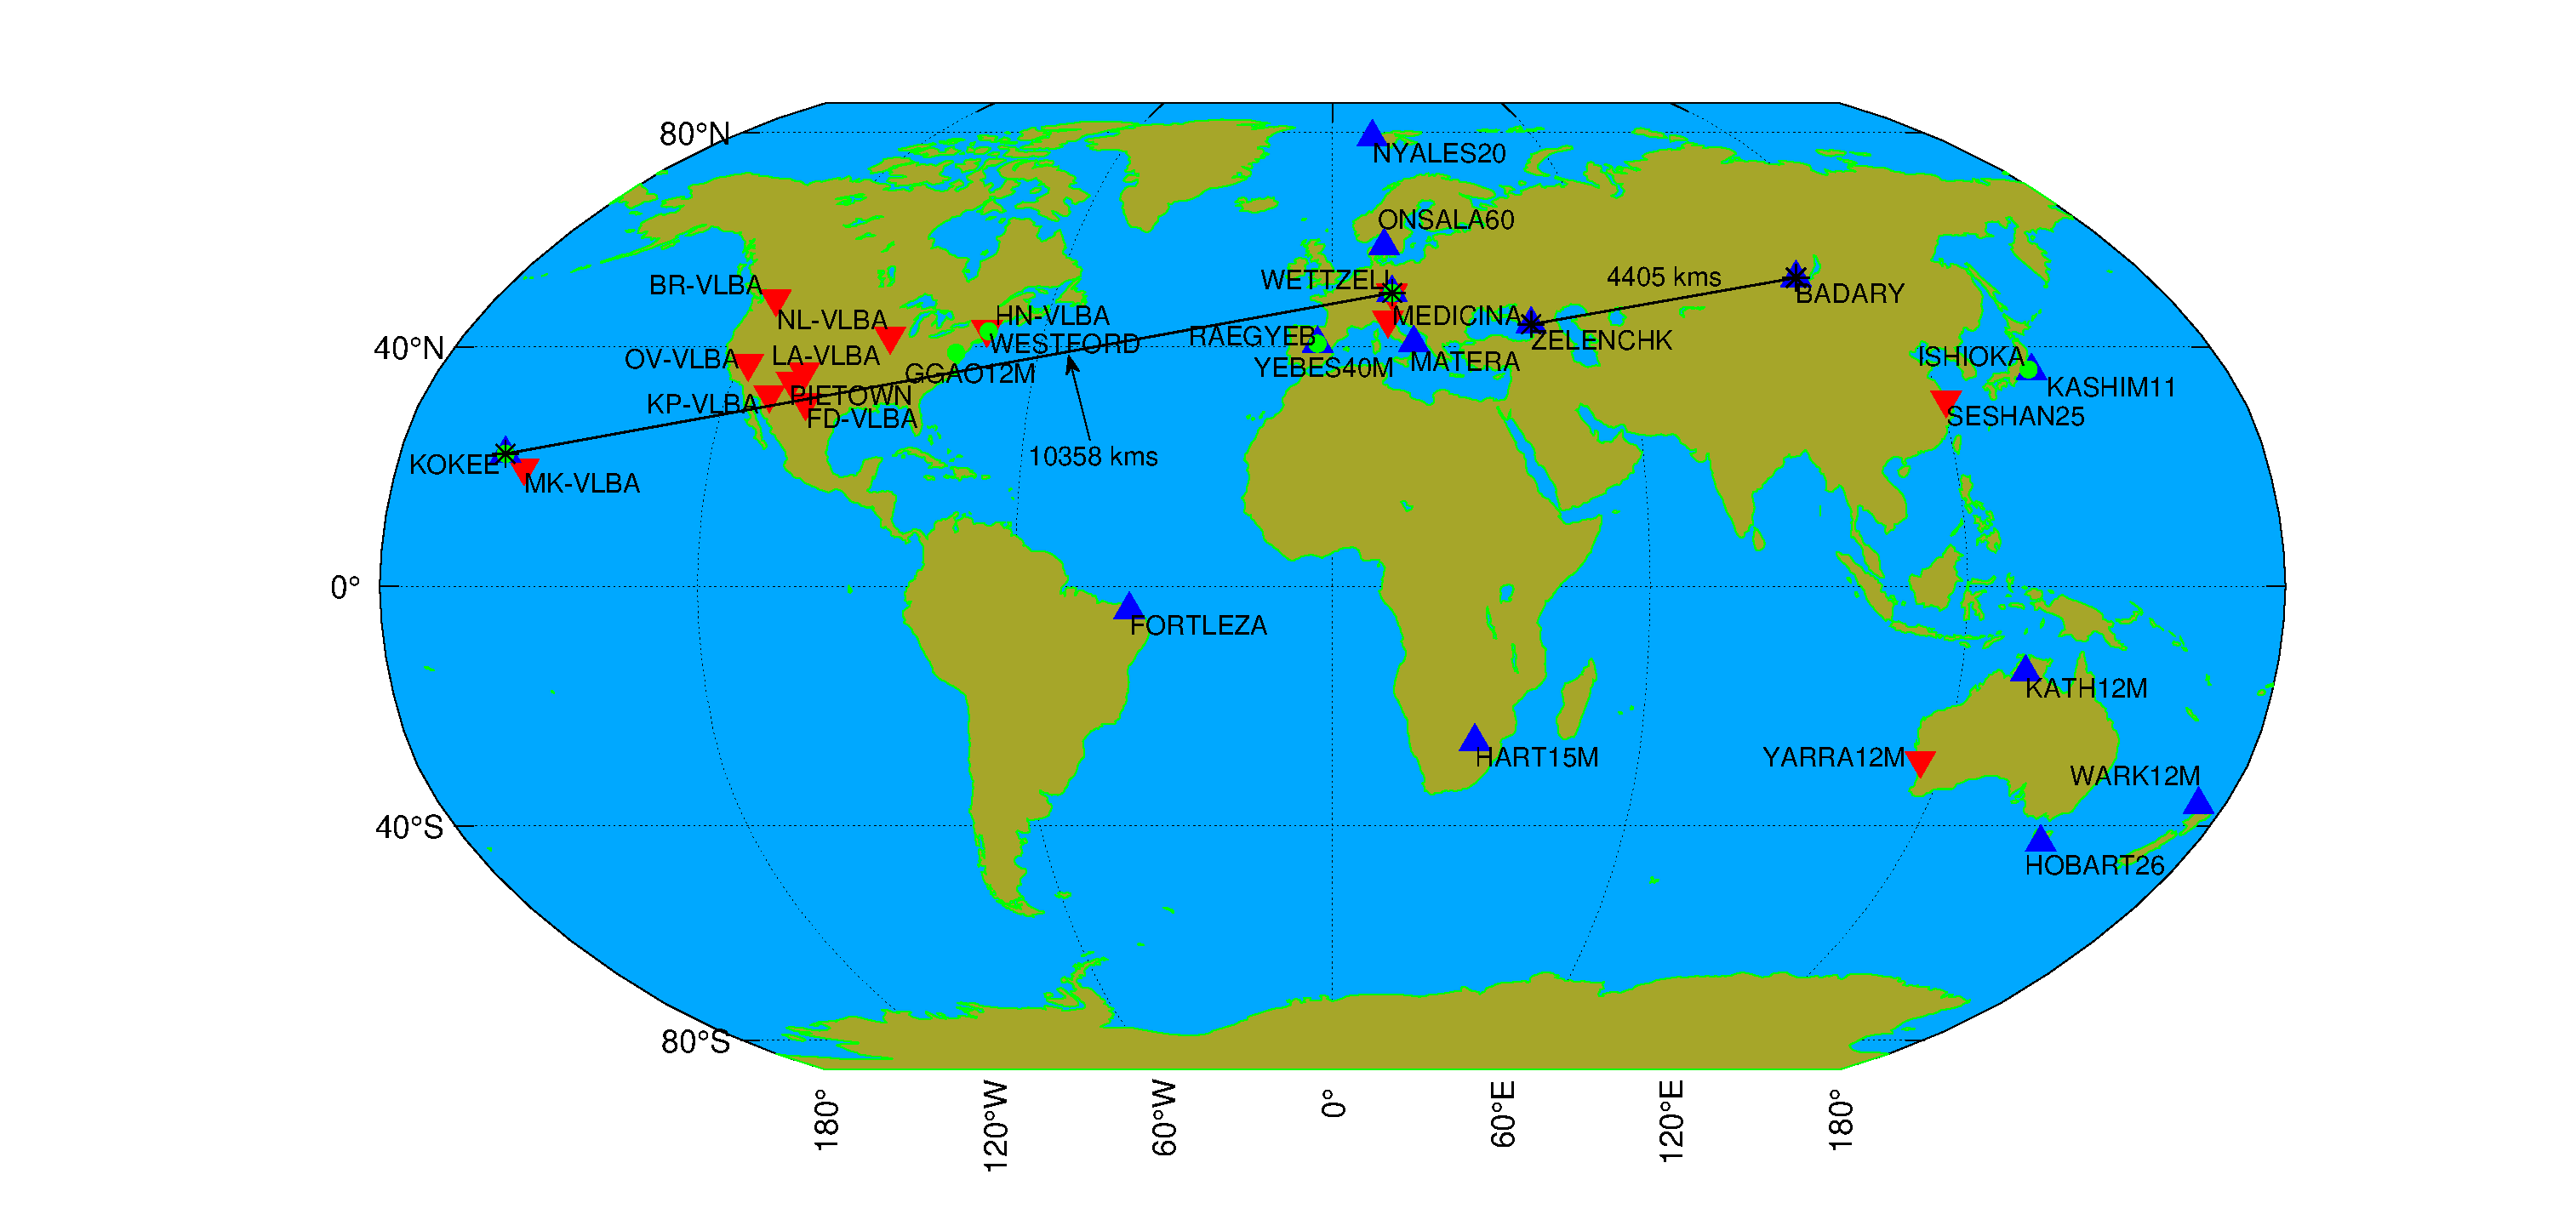
\includegraphics[scale=0.31]{VLBI_station_c.eps}
    \caption{Geographical representation of the stations of the various network. Legacy (S/X) stations in VLBA network (marked as the red triangle), IVS network (marked as the blue triangle); VGOS stations are represented by a Green circle; stations which participate in intensives are indicated by a black cross and their baselines are represented by a black solid line. \citep{rauteffect}}
    \label{fig:cont17stations}
\end{figure}
\begin{figure}
    \centering
    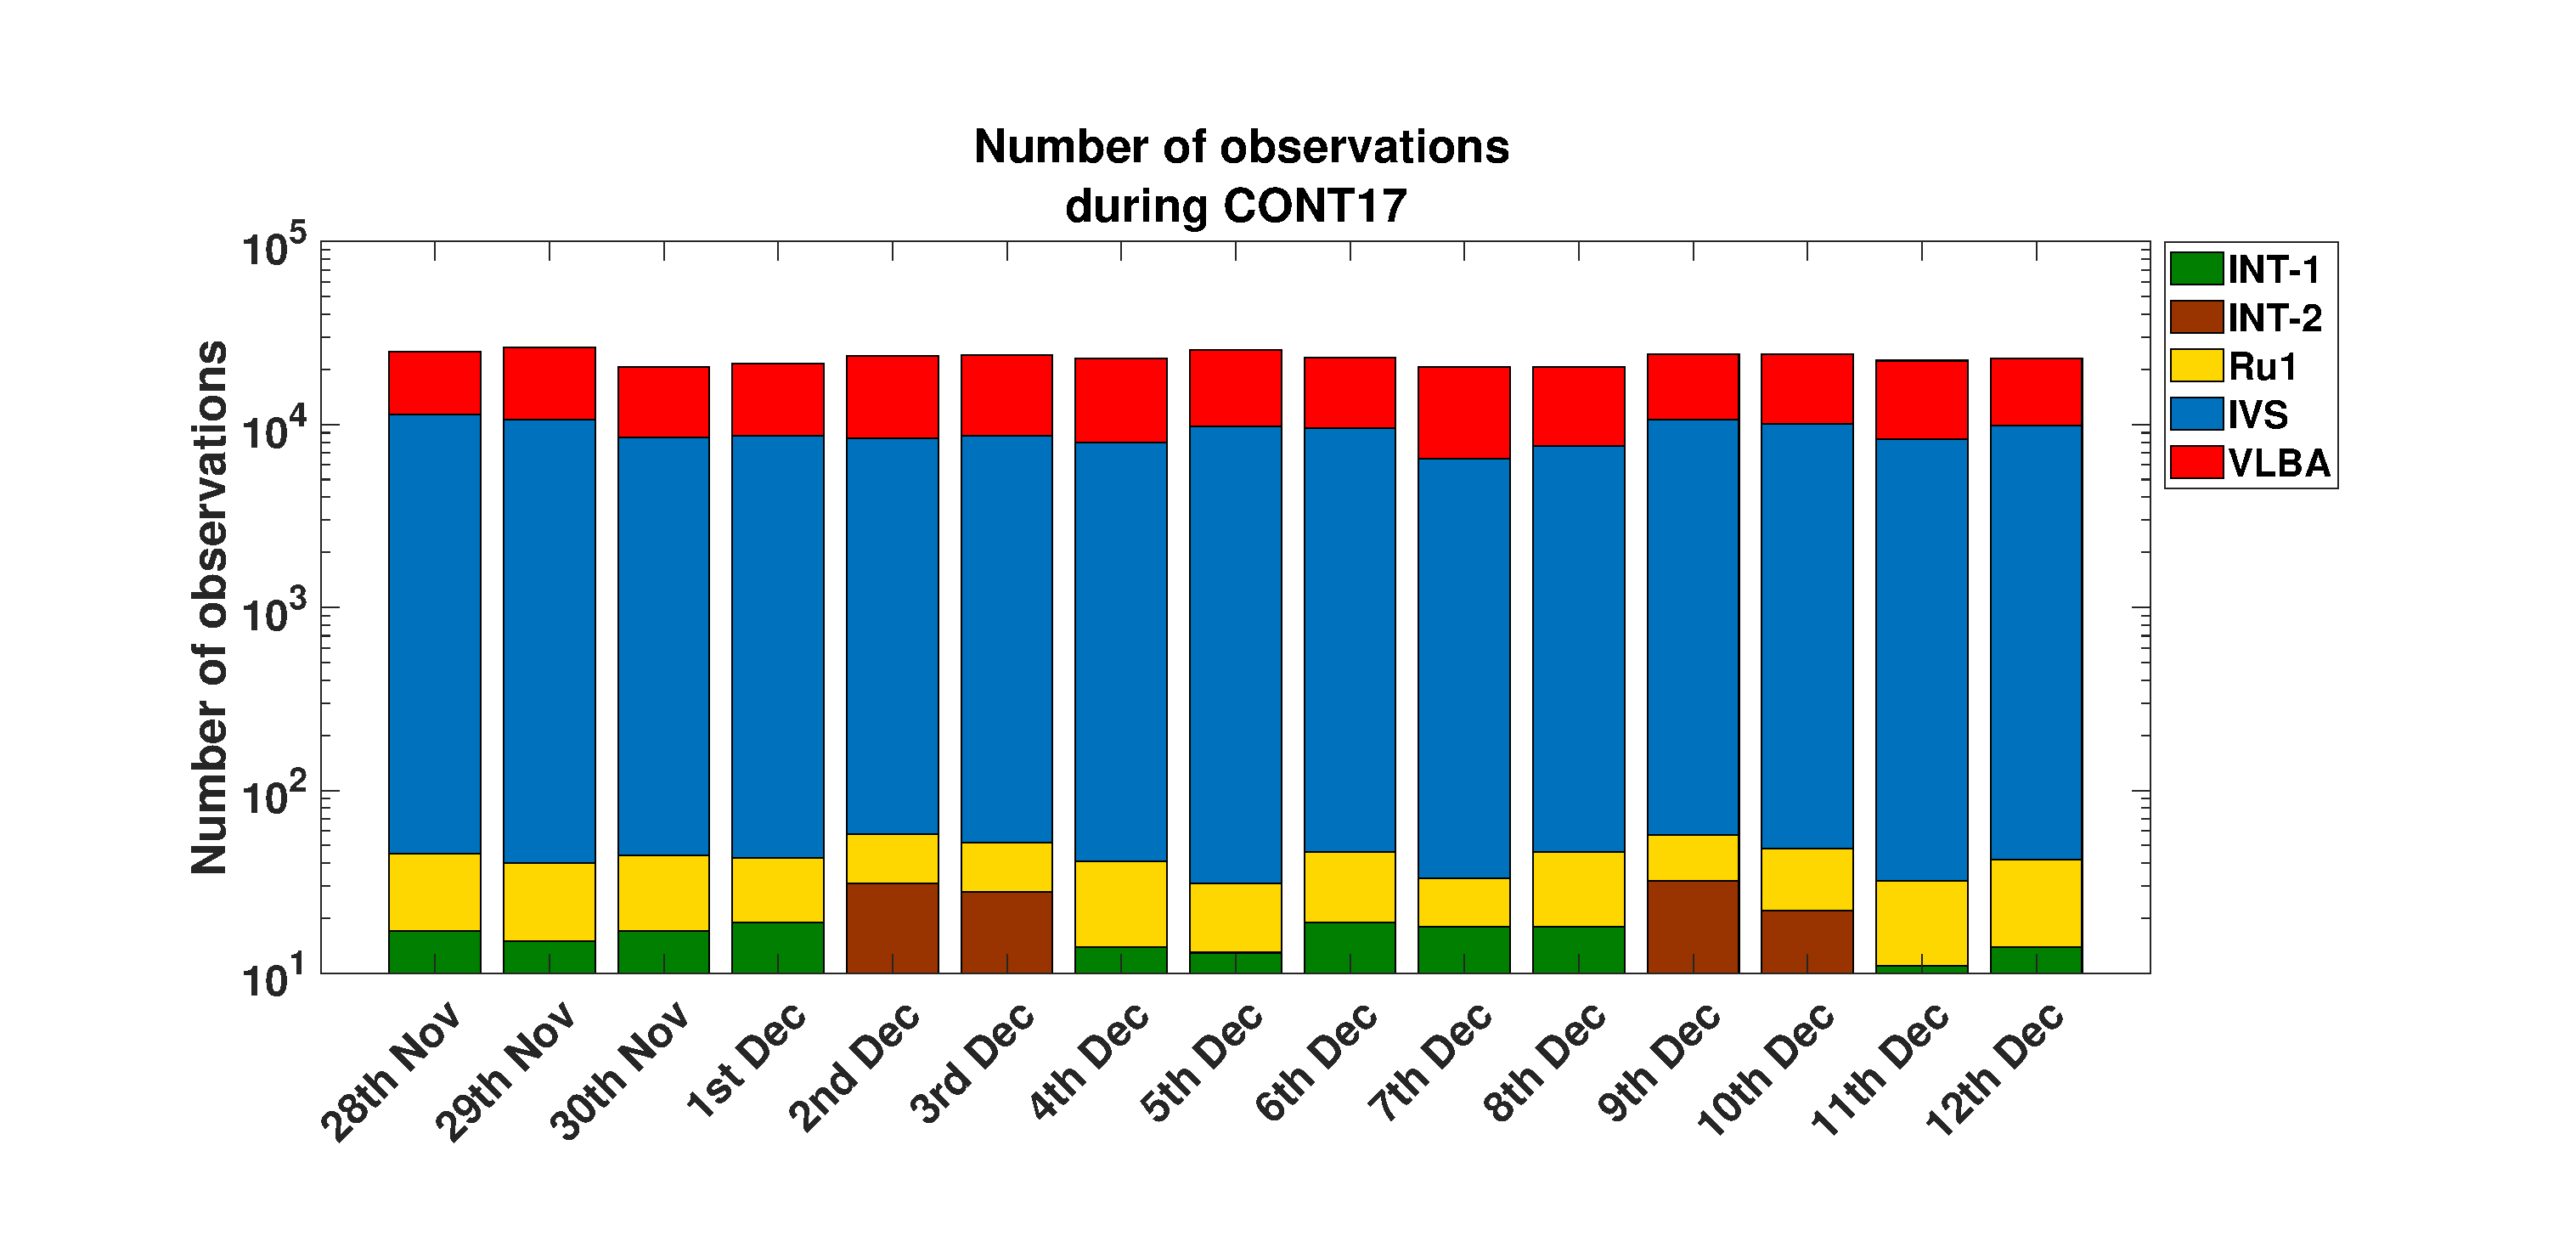
\includegraphics[scale=0.3]{noofobslog.eps}
    \caption{Number of VLBI observation during CONT17 campaign (observations from VGOS are not included). (\textit{y-axis has logarithmic scale})}
    \label{fig:noofobs}
\end{figure}


\section{DATA ANALYSIS}
The dUT1 from CONT17 data was estimated with VieVs@GFZ(\citep{nilsson2015application}. For our analysis, the models and the apriori used are shown in the table~\ref{tab:models}. At first, the dUT1 estimated from IVS, VLBA, and combined legacy networks were compared. The dUT1 was estimated for one day and 1-hour temporal resolutions. Here the standard parameterization for a 24-hour session was used (see table~\ref{tab:param}). Secondly, dUT1 from intensives is estimated, where the standard parameterization for Intensives was followed (see table~\ref{tab:param}). These estimated dUT1 values are compared with dUT1 values estimated from the legacy networks.
\begin{table}[]
\centering
\caption{A priori and correction models used for different parameters}
\label{tab:models}
\begin{tabular}{ccc}
\hline
\multicolumn{2}{c}{\textbf{Parameters}} & \textbf{Models/ Frames} \\ \Xhline{1pt}
\multirow{\textbf{Reference frames}} & Terrestial reference frame & ITRF2014 \\
 & Celestial reference frame & ICRF3 \\
\textbf{Ephimerides} & Ephimerides & JPL 421 \\
\multirow{\textbf{Troposphere}} & Pressure & GPT2 \\
 & Temperature & GPT2 \\
 & Mapping functions & Potsdam mapping function (PMF) \\
 & Gradients & APG (Bohm) \\
\textbf{Ionosphere} & Ionosphere delay & From NGS \\
\multirow{\textbf{Station models}} & Tidal Ocean loading & FES2004 \\
 & Tidal Atmosphere loading & vandam \\
 & Mean pole model & IERS 2015 \\
\multirow{\textbf{EOP}} & A priori time series & finals (Bulletin A) \\
 & Precession/Nutation model & IAU 2006/200A \\ \hline
\end{tabular}
\end{table}

\begin{table}[]
\caption{Standard parameterization used for analysing intensive and 24-hour VLBI sessions (*high relative constraint)}
\label{tab:param}
\centering
\begin{tabular}{|c|c|c|c|}
\hline
\multicolumn{2}{|c|}{\multirow{\textbf{Parameters}}} & \multicolumn{2}{c|}{\textbf{LSM parameterization}} \\ \cline{3-4} 
\multicolumn{2}{|c|}{} & \textbf{Intensives} & \textbf{24-hour} \\ \hline
\multirow{\textbf{\begin{tabular}[c]{@{}c@{}}Troposphere \\ \\ Estimation\end{tabular}}} & Zenith wet delays & Estimated & Estimated \\ \cline{2-4} 
 & North gradients & Not Estimated & Estimated \\ \cline{2-4} 
 & East gradients & Not Estimated & Estimated \\ \hline
\textbf{Clock Estimation} &  & Estimated & Estimated \\ \hline
\multirow{\textbf{EOP}} & x-pole & Not Estimated & Estimated \\ \cline{2-4} 
 & y-pole & Not Estimated & Estimated \\ \cline{2-4} 
 & UT1-UTC & Estimated* & Estimated \\ \cline{2-4} 
 & nutdx & Not Estimated & Estimated \\ \cline{2-4} 
 & nutdy & Not Estimated & Estimated \\ \hline
\textbf{Station Coordinates} &  & Not Estimated & Estimated \\ \hline
\textbf{Source Coordinates} &  & Not Estimated & Estimated \\ \hline
\end{tabular}
\end{table}

\section{RESULTS}
\subsection{dUT1 from 24-hour sessions}
The dUT1 time-series was estimated from 24-hour sessions of IVS, VLBA, and combined network (IVS + VLBA) using global solutions in VieVs@GFZ software. The model/apriori data, and parameterization were used as given in table~\ref{tab:models} and~\ref{tab:param}, respectively. The dUT1 were estimated for one day and one-hour resolution. \\
As we can see from the figure~\ref{fig:dut1} that dUT1 estimated from the combined network has approximately average values of dUT1 estimated from individual legacy networks, for both resolutions. The dUT1 from combined networks also has smaller formal errors and fewer outliers. This can be explained as the combined network has significantly more observations and participating stations. The hourly dUT1 contains sub-daily variations which can be seen in the bottom figure~\ref{fig:dut1}. To understand the relationship between dUT1 estimated from IVS and VLBA network, we computed the correlation between them. For one day resolution, the correlation was found to be 0.93 and for one-hour resolution, it is 0.61. The decrease in correlation coefficient for hourly resolution might be due to different sub-daily variations in the legacy networks. 
To summarize, dUT1 estimated from combined and individual legacy networks are consistent with each other. \\
\begin{figure}[h]
    \centering
    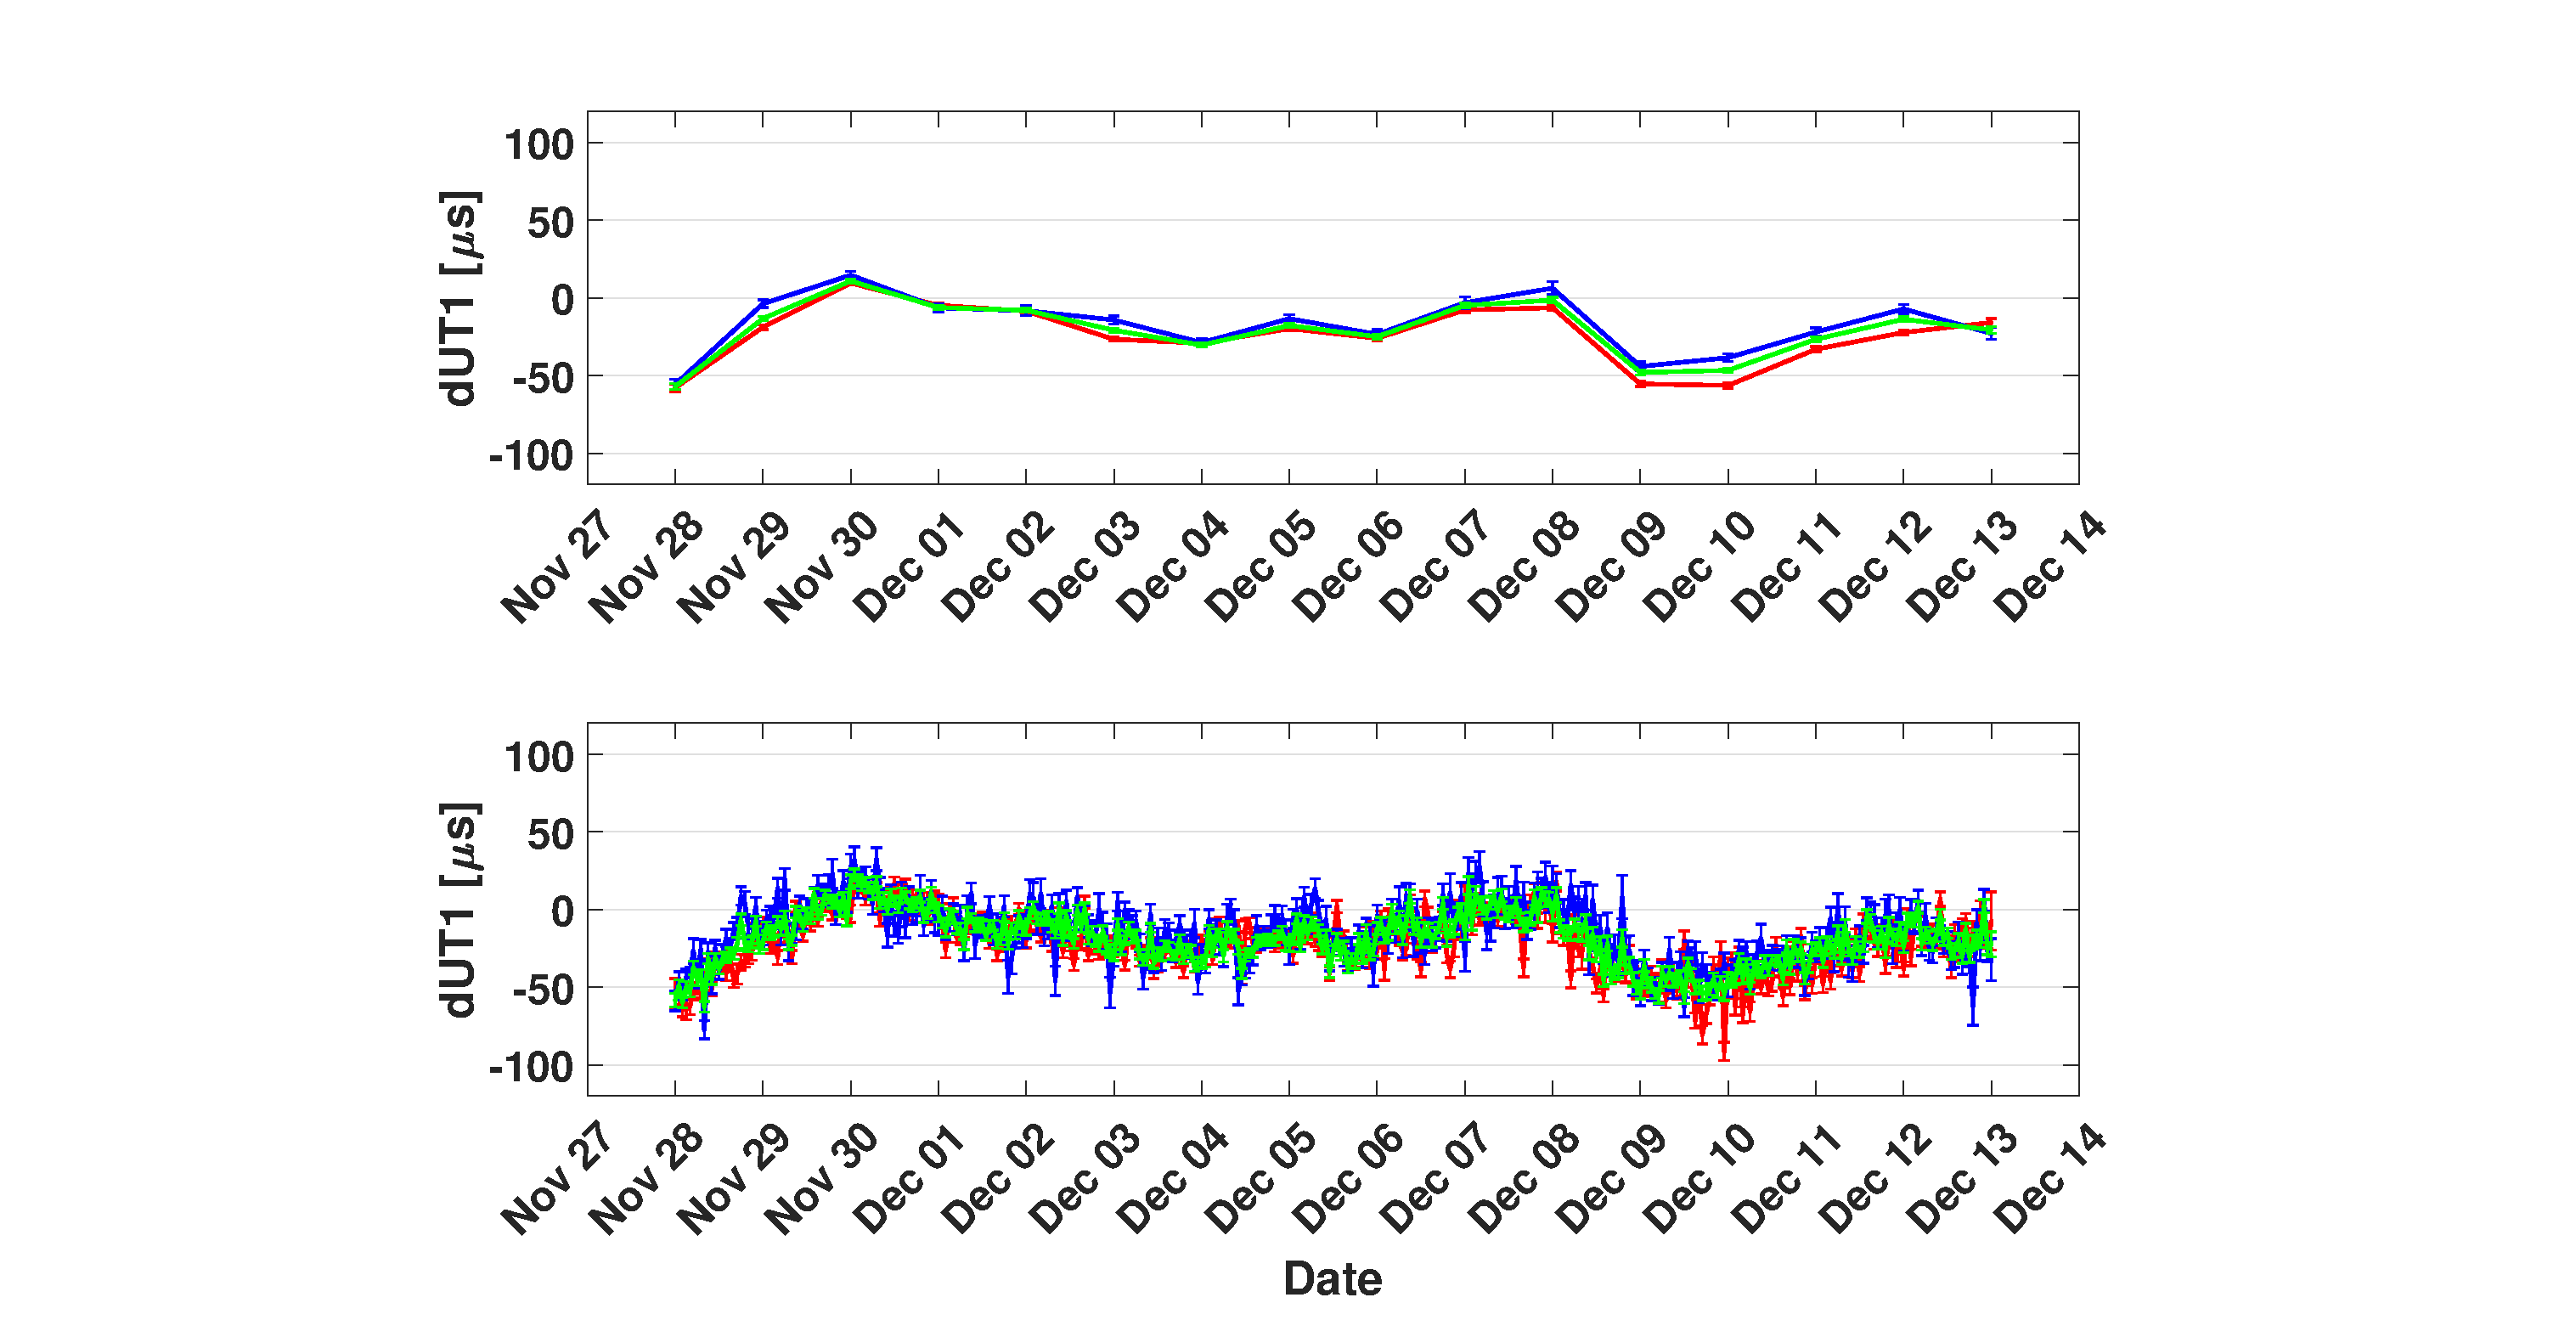
\includegraphics[scale=0.3]{dut1.eps}
    \caption{dUT1 estimates for 1 day (top) and 1-hour (below) resolution; The blue, red and green line represents dUT1 estimated from IVS, VLBA and combined network, respectively.}
    \label{fig:dut1}
\end{figure}
\begin{table}[h]
\centering
\caption{The root mean square (RMS) values of the dUT1 estimates from 3 networks and their corresponding mean errors. 
(All values are in $\mu secs$)}
\label{tab:rmsdut1}
\begin{tabular}{ccccc}
\hline
Networks & \multicolumn{2}{c}{1 day} & \multicolumn{2}{c}{1 hour} \\ \hline
(in $\mu secs$) & \begin{tabular}[c]{@{}c@{}}RMS of\\ Estimates\end{tabular} & \begin{tabular}[c]{@{}c@{}}Mean\\ Error\end{tabular} & \begin{tabular}[c]{@{}c@{}}RMS of\\ Estimates\end{tabular} & \begin{tabular}[c]{@{}c@{}}Mean\\ Error\end{tabular} \\ \Xhline{1.2}
IVS & 24.70 & 2.97 & 23.94 & 7.63 \\
VLBA & 30.34 & 1.62 & 28.54 & 4.48 \\
Combined & 27.17 & 1.47 & 25.06 & 3.76 \\ \hline
\end{tabular}
\end{table}

\subsection{dUT1 from Intensive sessions}
Now we will compare dUT1 values from intensive sessions with dUT1 estimated from legacy networks. The daily dUT1 values from the 3 intensive networks are over-plotted with dUT1 from IVS and VLBA networks at 00:00:00 UTC epoch. As the IVS-INT1 and IVS-INT2 have the same baselines with different observing time and observed sources, they are grouped for this dUT1 over-plot, and dUT1 from Russian intensives are plotted separately for our analysis. \\
It can be observed from the figure~\ref{fig:dut1int}, that the dUT1 values from intensives do not show a good agreement with daily dUT1 values from legacy networks. To further validate the relationship between them, the correlation coefficient is computed. The coefficient between IVS intensives and Legacy networks is near to zero and hence no correlation was found between them. This could be due to different observing times of IVS-INT1 (evening) and IVS-INT2 (morning), it might have resulted in inconsistent dUT1 values. However, the correlation coefficient between Russian intensives and IVS, and VLBA are 0.62 and 0.68 respectively, which considerably shows better agreement between them. The possible reason can be explained as most parameters are not estimated, i.e., fixed to a priori values when estimating dUT1 from intensives. The inaccuracies present in the a priori values of the fixed parameters, it will further propagate in the dUT1 determination. In addition to the reason mentioned above, the inconsistencies between the dUT1 values could be present due to the different observing times. The estimated daily values of dUT1 from intensive sessions are computed from observations that span approximately one hour during a day, the sub-daily variations in dUT1 might be present in it. The sub-daily variations in daily dUT1 from legacy networks are not present as these variations are averaged out in such 24-hour sessions. This might be another possible reason for the inconsistencies present between the dUT1 estimated from intensives and legacy networks. To improve the agreement between them, we can compare the dUT1 values for the same interval. \\
\begin{figure}[h]
    \centering
    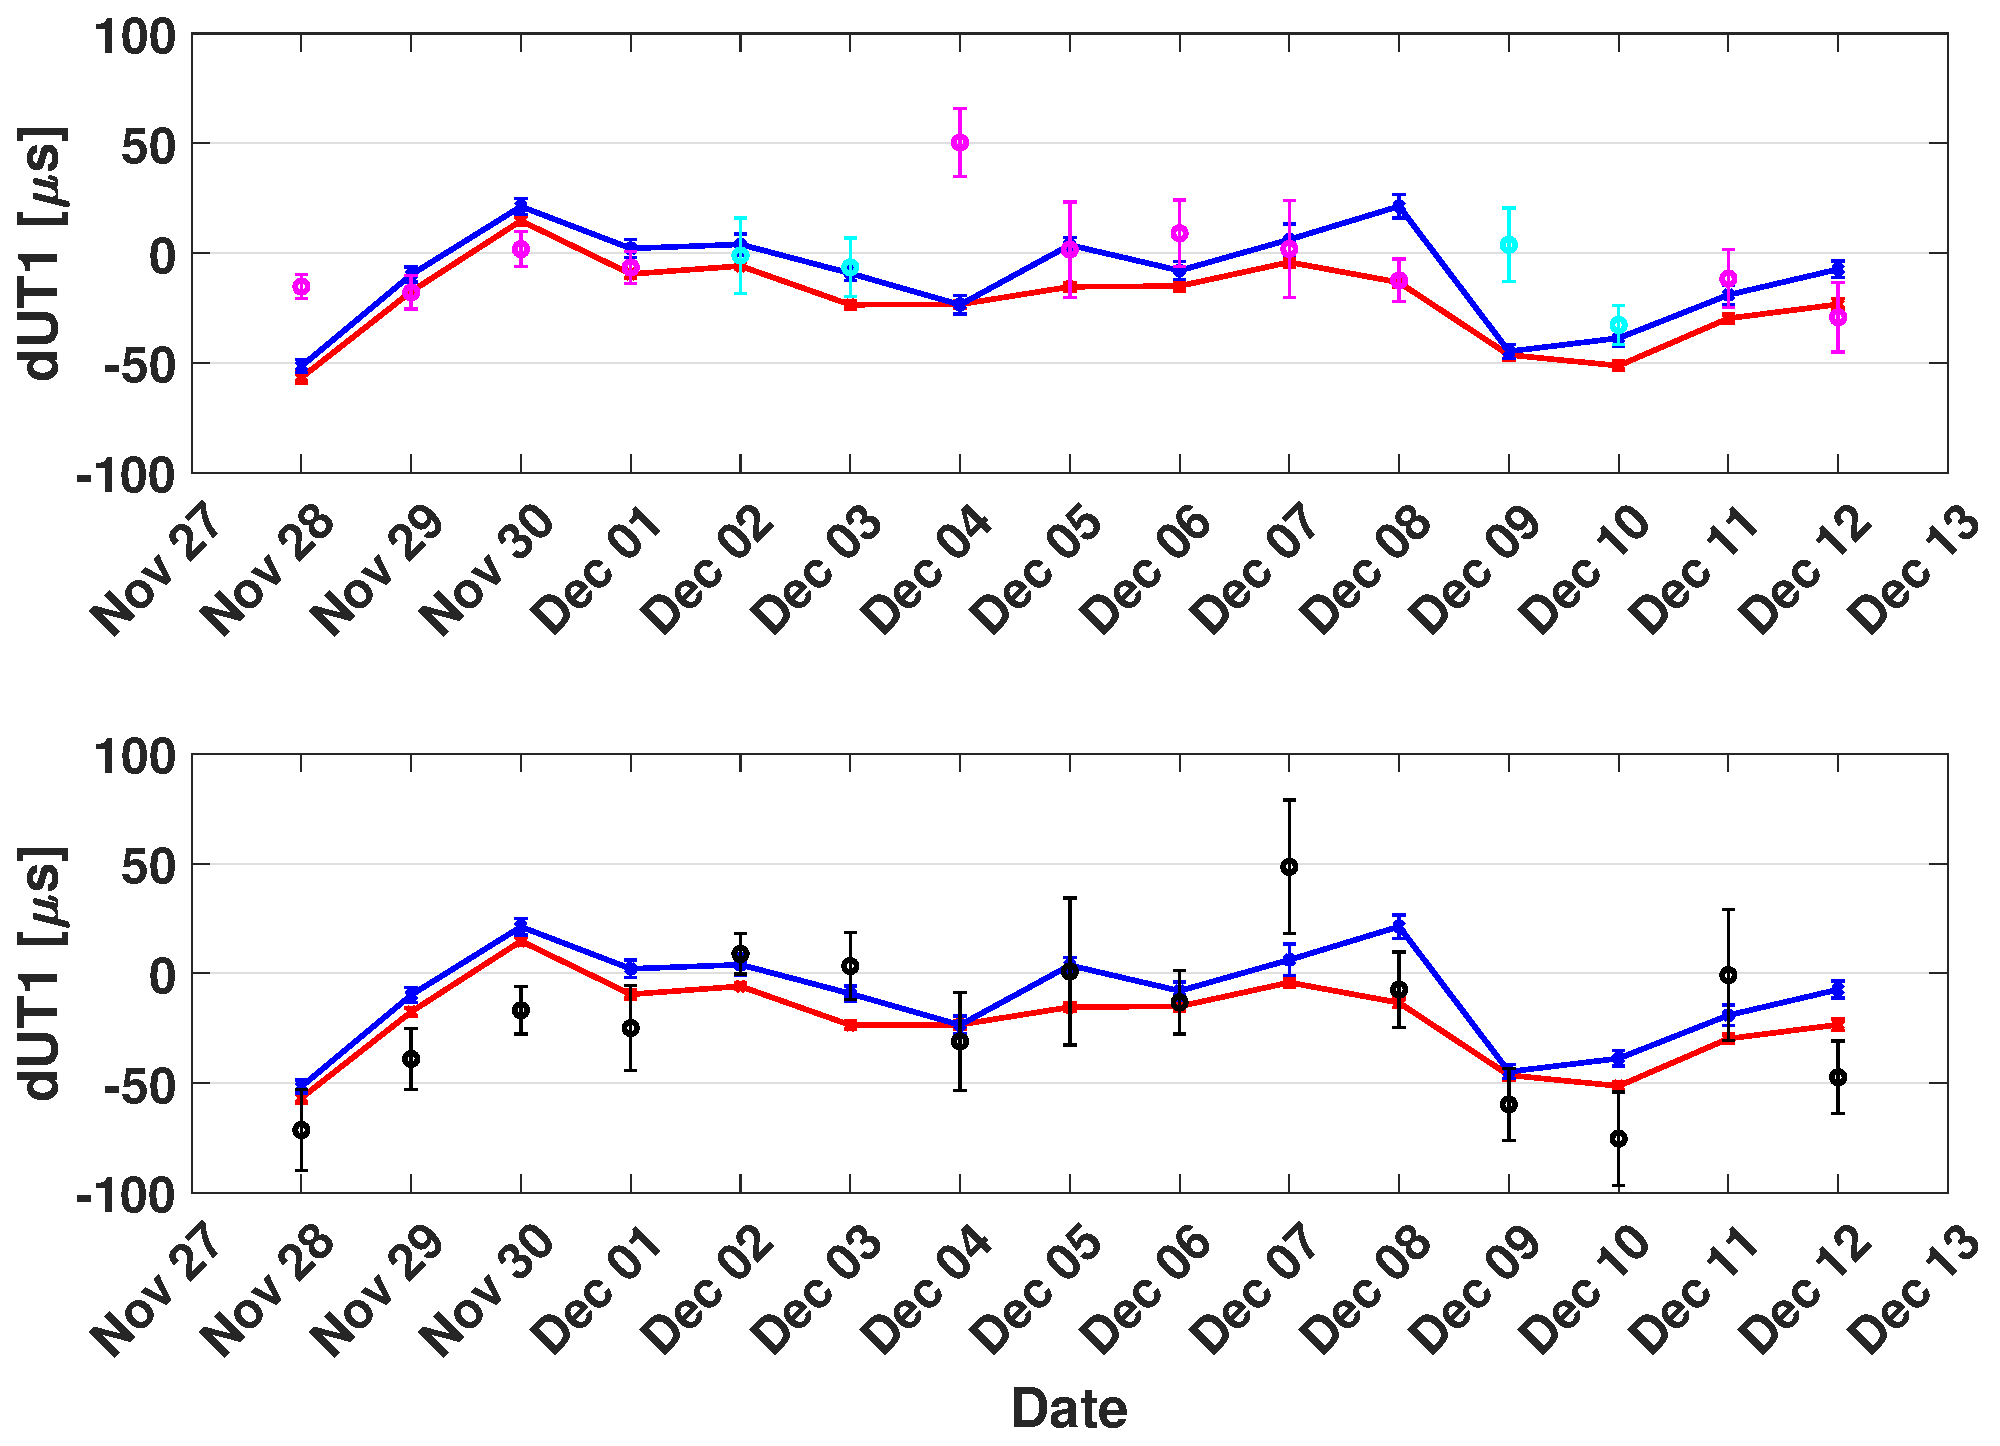
\includegraphics[scale=.28]{dut11day.eps}
    \caption{Comparison of daily dUT1 estimates from Legacy networks with IVS intensives (top) and Russian intensives (bottom). \textit{Blue and Red lines represents IVS and VLBA networks respectively; Magenta, cyan, and black represents dUT1 from IVS-INT1, IVS-INT2, and Russian intensives respectively}.}
    \label{fig:dut1int}
\end{figure}
This comparison can be done with two approaches. The first approach is to estimate the dUT1 from 24-hour sessions for an hourly resolution. Then we can compare dUT1 from the intensive session with the hourly dUT1 estimated from legacy networks for the corresponding interval when the intensive session took place. The other approach is to compute the dUT1 value from the intensive session and then extrapolate this value to the nearest midnight epoch (i.e., 00:00:00 UTC) using high-frequency EOP models. This dUT1 value can be compared to the daily dUT1 value estimated from the legacy networks. \\
In the first approach, we compare the dUT1 of the mean epoch of the intensive session. For example, if the intensive session spans from 18:30 to 19:30, we compare with dUT1 value at the 19:00 epoch. The figure~\ref{fig:dut1int1hr} displays this comparison. It is difficult to infer strongly from the figure~\ref{fig:dut1int1hr}, whether dUT1 shows better agreement with hourly dUT1 than daily dUT1 from legacy networks. To understand better, we computed the root mean square value of the difference in dUT1 estimates from intensive and legacy networks. As we can see from the figures~\ref{fig:rmsdut1xb} and~\ref{fig:rmsdut1xa}, we can infer that dUT1 from IVS-INT1 network shows slightly better agreement with the hourly dUT1 from the legacy networks. On the contrary, dUT1 from IVS-INT2 and Russian network do not show any improvement. The reason for this is not clear at the moment.
\begin{figure}[h]
    \centering
    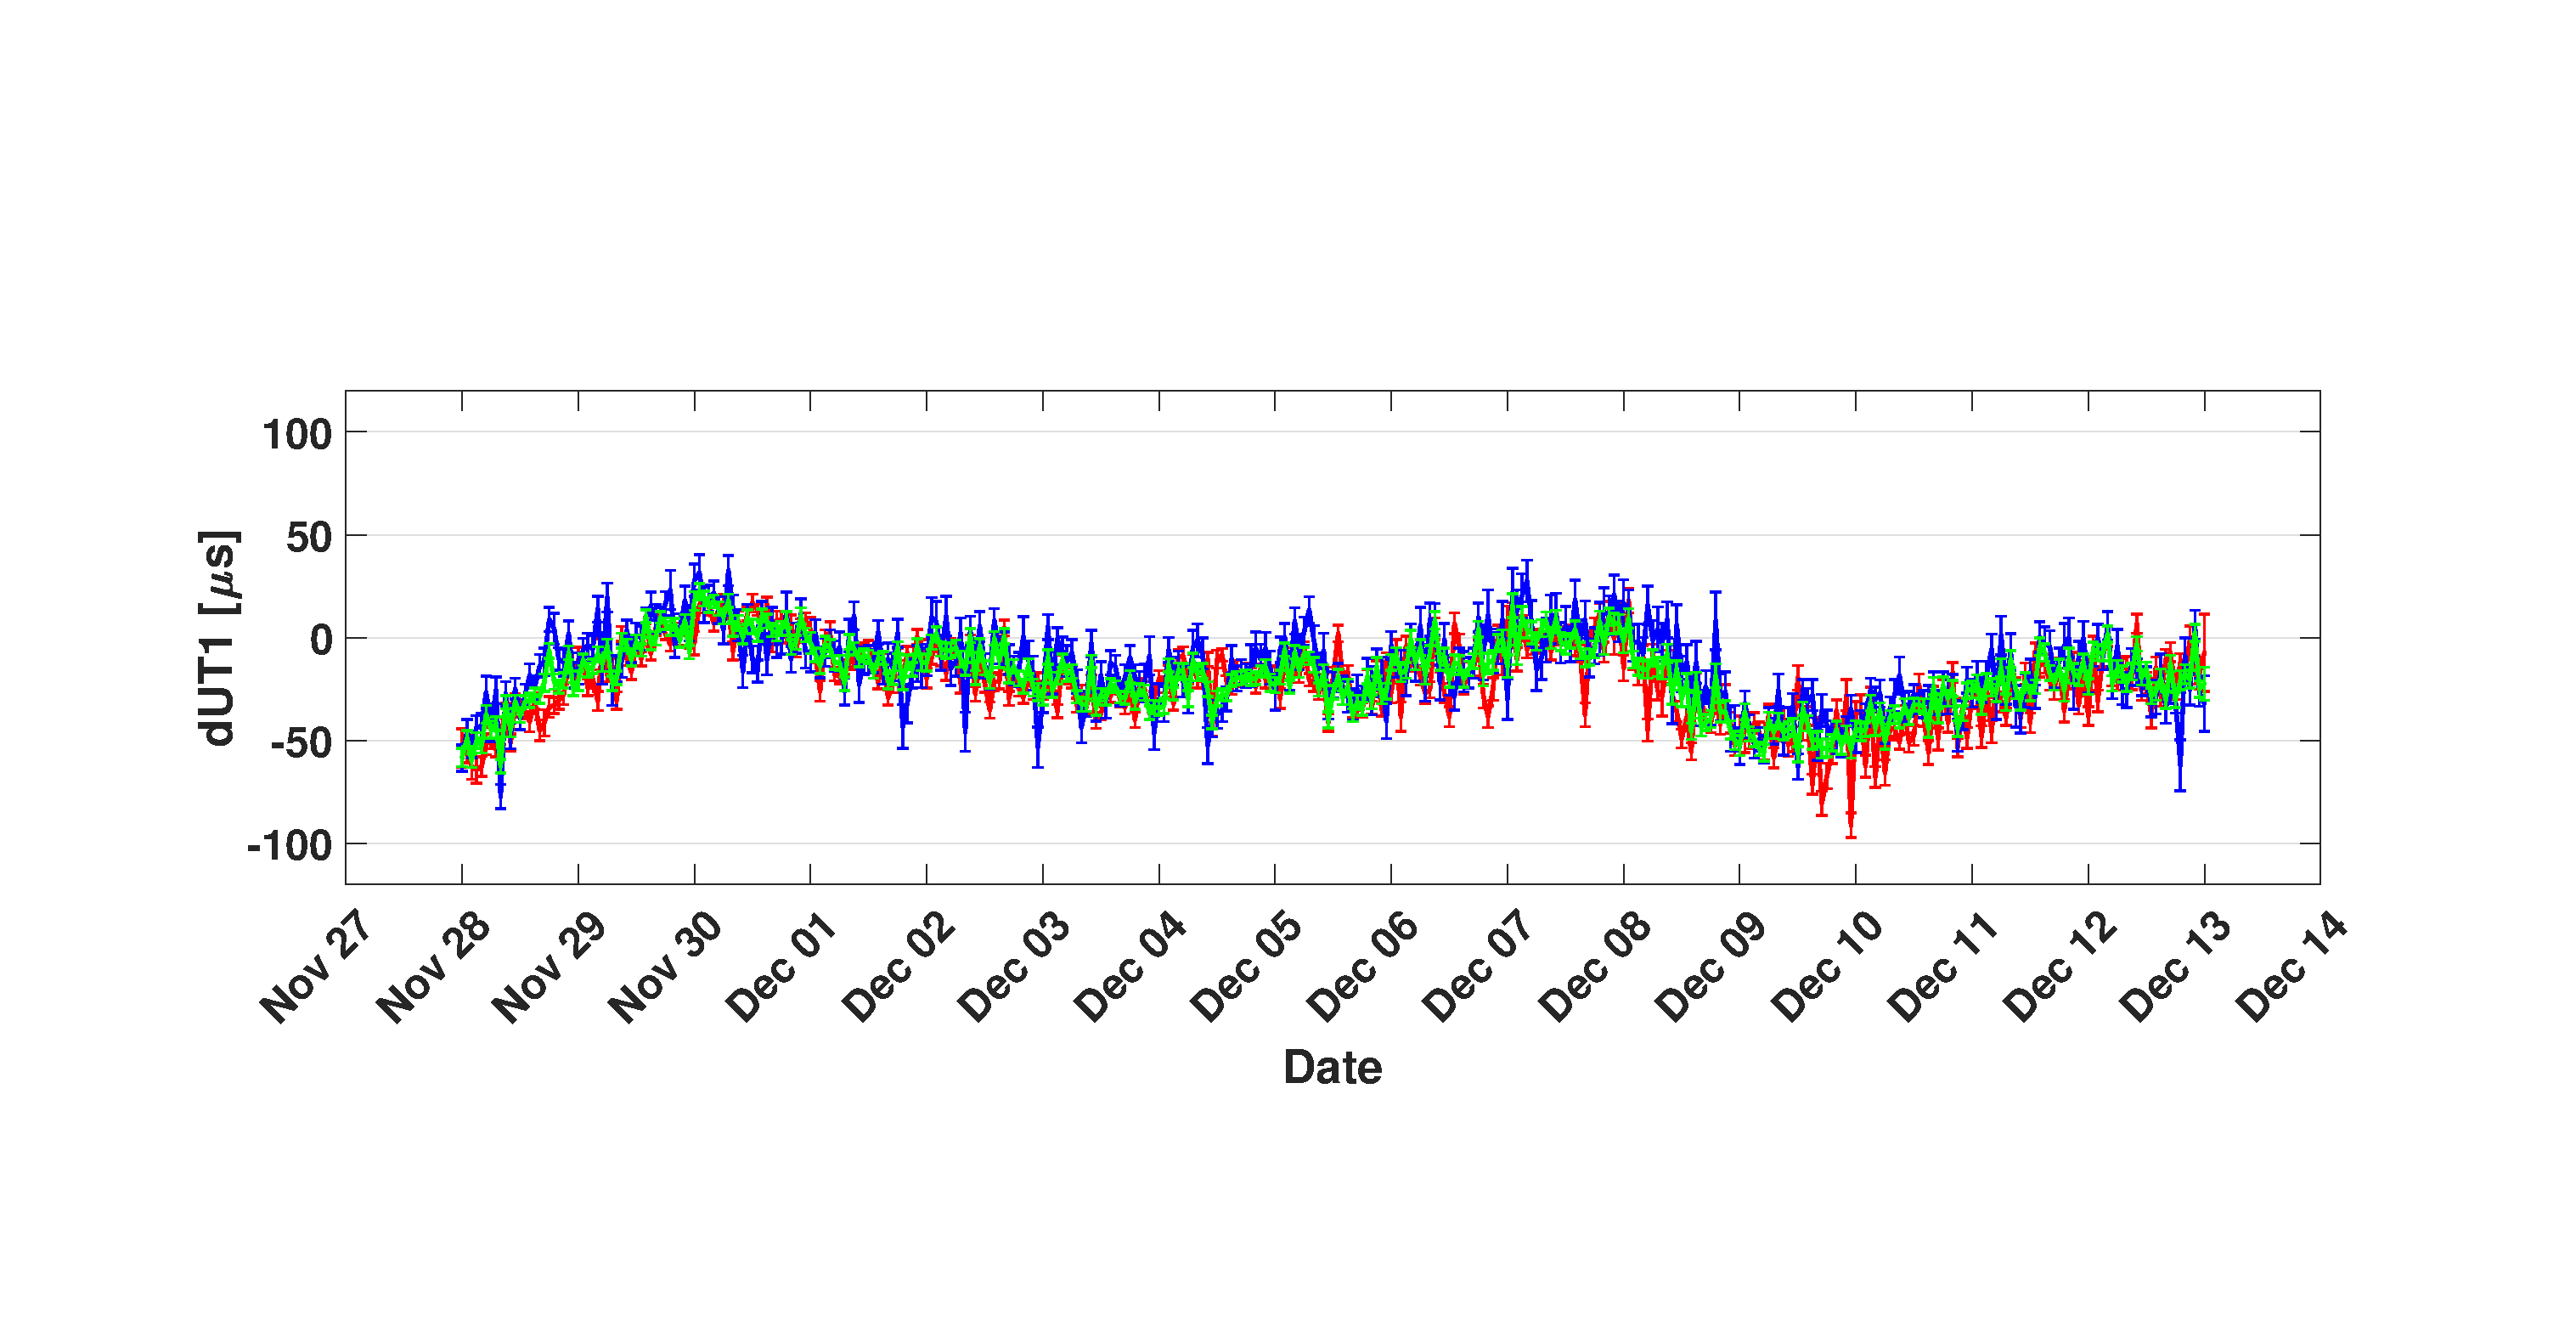
\includegraphics[scale=.28]{dut1hr.eps}
    \caption{Comparison of hourly dUT1 estimates from Legacy networks with IVS intensives (top) and Russian intensives (bottom). \textit{Blue and Red lines represents IVS and VLBA networks respectively; Magenta, cyan, and black represents dUT1 from IVS-INT1, IVS-INT2, and Russian intensives respectively}.}
    \label{fig:dut1int1hr}
\end{figure}

\begin{figure}[h]
    \centering
    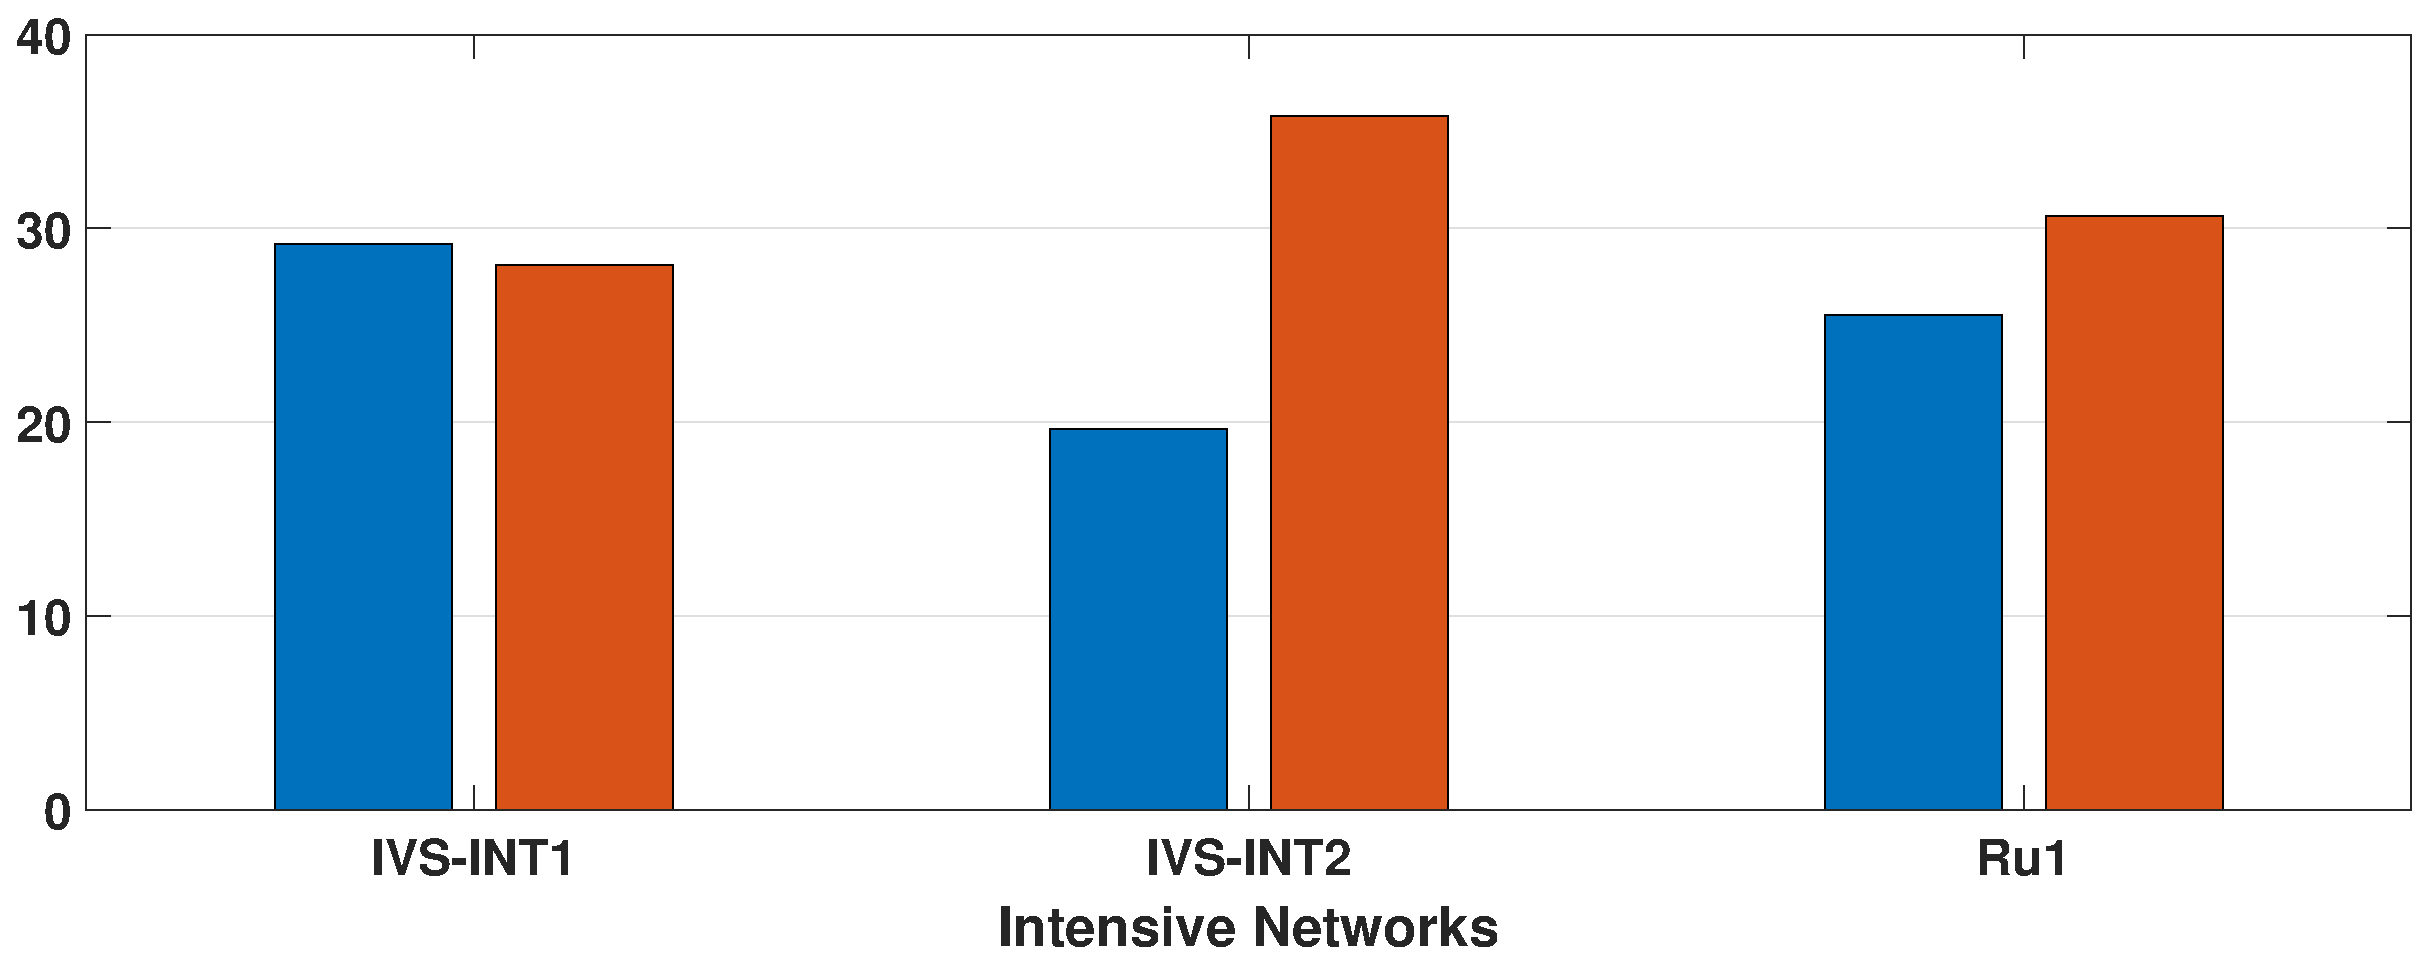
\includegraphics[scale=0.25]{rmsdut1xb.eps}
    \caption{The root mean square value of the difference between dUT1 estimated from IVS network and intensive networks; Blue and red coloured bar represents difference in dUT1 for daily and hourly resolution, respectively.}
    \label{fig:rmsdut1xb}
\end{figure}

\begin{figure}[h]
    \centering
    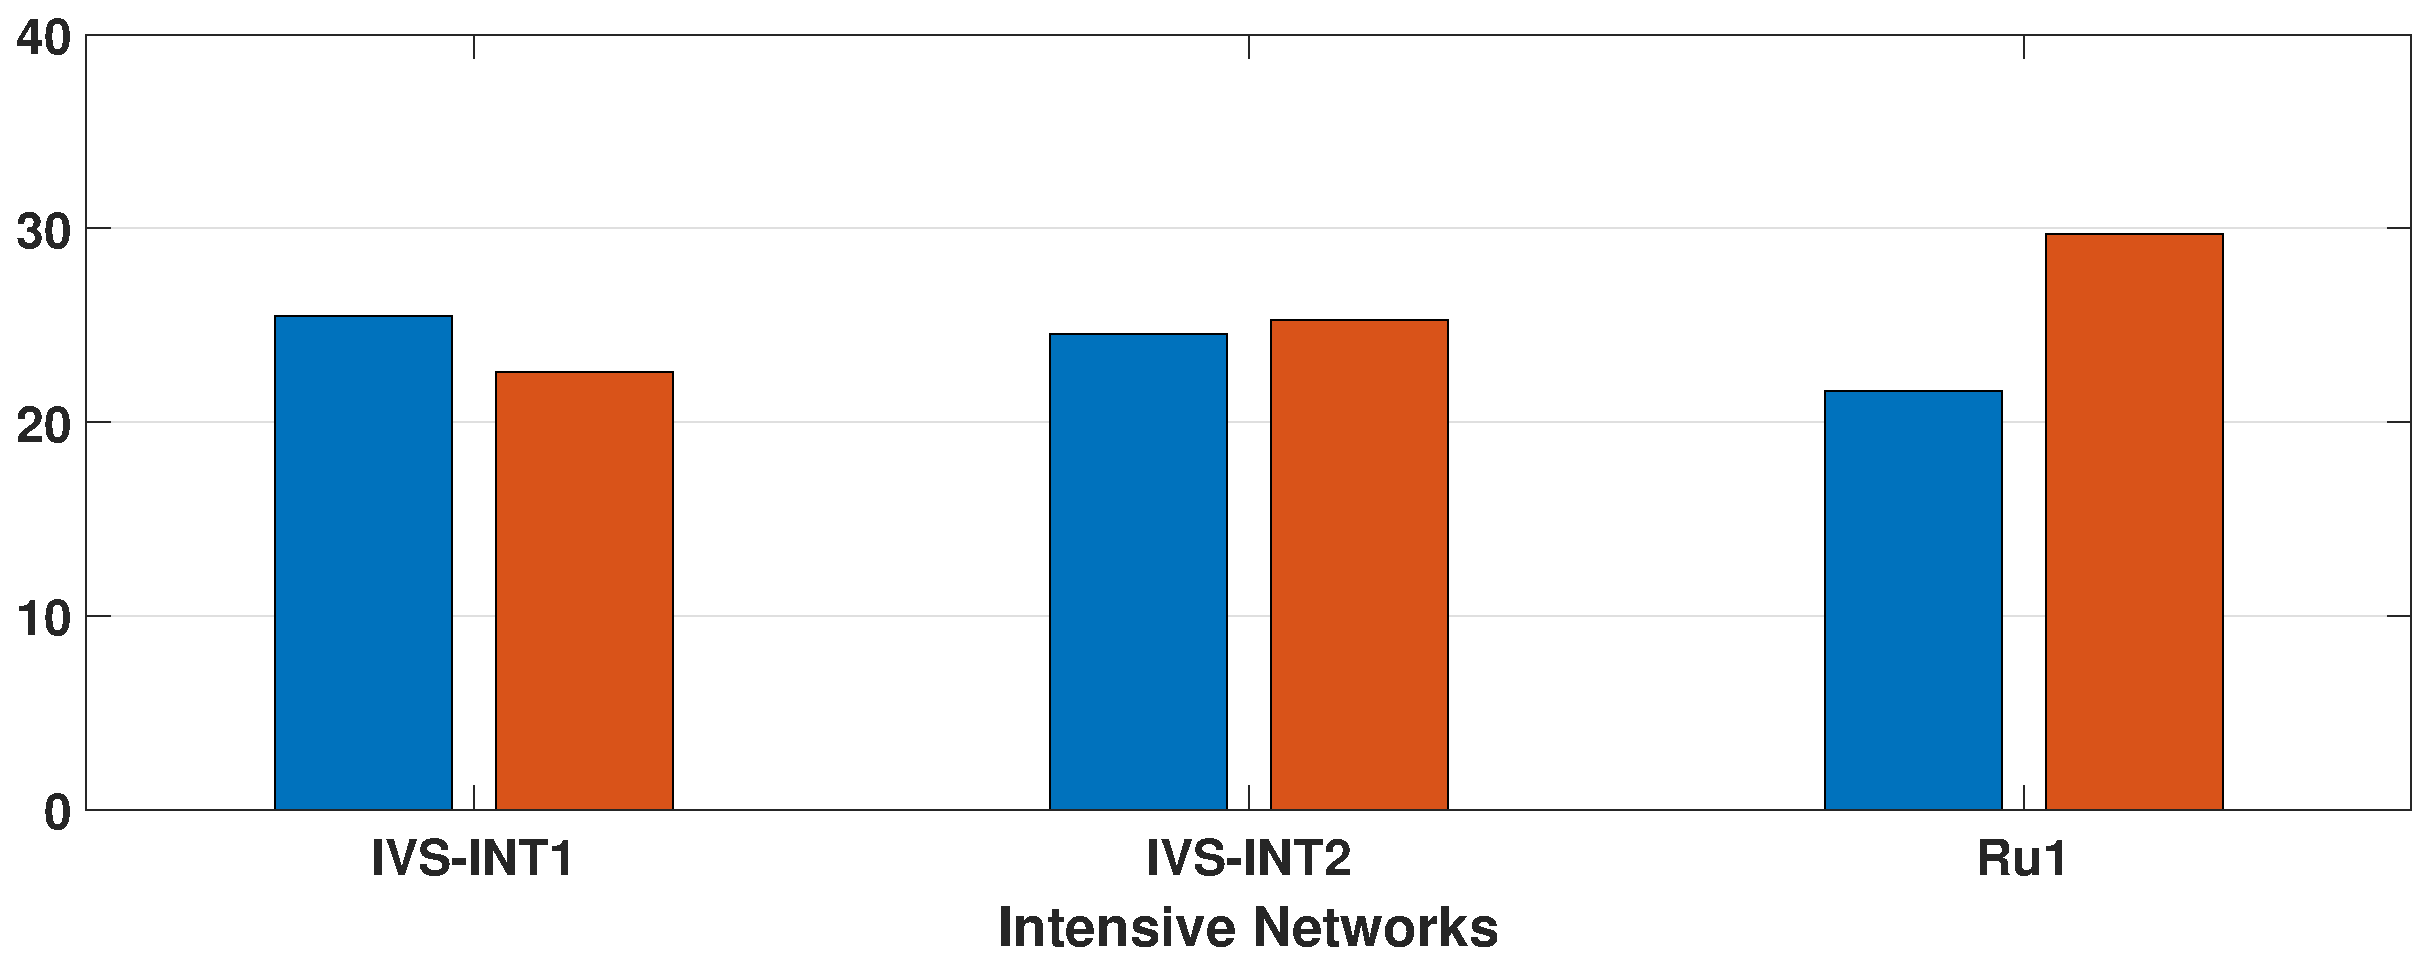
\includegraphics[scale=0.25]{rmsdut1xa.eps}
    \caption{The root mean square value of the difference between dUT1 estimated from VLBA network and intensive networks; Blue and red coloured bar represents difference in dUT1 for daily and hourly resolution, respectively.}
    \label{fig:rmsdut1xa}
\end{figure}

\section{CONCLUSIONS}
%\begin{acknowledgements}
%If you'd like to thank anyone, place your comments here
%and remove the percent signs.
%\end{acknowledgements}

% BibTeX users please use one of
% \bibliographystyle{spbasic}      % basic style, author-year citations
% %\bibliographystyle{spmpsci}      % mathematics and physical sciences
% %\bibliographystyle{spphys}       % APS-like style for physics
% %\bibliography{}   % name your BibTeX data base

% % Non-BibTeX users please use
% \begin{thebibliography}{}
% %
% % and use \bibitem to create references. Consult the Instructions
% % for authors for reference list style.
% %
% \bibitem{RefJ}
% % Format for Journal Reference
% Author, Article title, Journal, Volume, page numbers (year)
% % Format for books
% \bibitem{RefB}
% Author, Book title, page numbers. Publisher, place (year)
% % etc
% \end{thebibliography}
\bibliography{reference}
\bibliographystyle{spbasic}
\end{document}
% end of file template.tex